% This chapter presents a survey of patrolling, surveillance, navigation and exploration strategies already implemented in the literature. In the last decades, related algorithms for multiple robot teams have piqued the interest of the robotics community, becoming a remarkable growing area. One of the main reasons contributing to this fact is the variety of approaches that these algorithms can comprise. Many authors contributed with studies that involve many different strategies to solve these problems. In this section, some of the background work related to different strategies is presented. The reader will note that it is not imperative to follow just one of these strategies. In fact, most of them result from mixed strategies, though more evident characteristics related to the strategy being discussed are focused in each section.
% <---- Real-time tracking systems ---->

This section presents an overview of \acs{IoT} connected healthcare applications. (...) \bigskip
%==========================================================================================================================================
%[1] P. Fuhrer and D. Guinard, “Building a smart hospital using RFID technologies,” Eur. Conf. eHealth 2006, Proc. ECEH 2006, pp. 131–142, 2006.
%
%--------------------------
% Physiological & Environmental Signals: (L1) 
% - RFID tag
% Networking Protocols: (L2)
% - RFID (EPC Gen1?), WiFi
% Gateway: (L3)
% - Beaglebone Black
% Data Storage: (L4)
% - MySQL
% e-Health Standards: (L5)
% - None
% Application Features: (L6)
% - Real-Time Tracking System (Patients and Assets)
% Security:
% - Unknown Storage Encryption 
% User Interface:
% - Custom Web application
% Other Notes: 
%------------------------------

In \cite{Fuhrer2006}, one of the first \acs{IoT} applications for healthcare is described. The authors propose a real-time locating system (RTLS) using \acs{RFID} tags called RFIDLocator. These tags are placed in hospital equipment, staff, patients and medical files and using \acs{RFID} readers placed in strategic locations around the hospital (\textit{e.g.} entrance of rooms, handheld readers), it is possible to track the location of each object. When a \acs{RFID} reader detects a \acs{RFID} tag it communicates this information, using Wi-Fi, to a central server which stores it in a MySQL database. Healthcare workers can then view this information through a web application, which contains a location history of the tagged object. The authors show how RTLS systems can mitigate the risks of patient misidentification, loss or theft of assets and even drug counterfeiting. However, in this article, security and privacy issues are not discussed. Although not stated explicitly, communications between the RFID tags and the RFID readers are assumed to be unencrypted, which means ``unethical individuals could snoop on people and surreptitiously collect data (...) without their knowledge'', even after leaving the hospital if the tags are not removed. This raises serious privacy concerns, as the tags could contain private information that can be detrimental to the patients if revealed. \bigskip

%==========================================================================================================================================
%[2] T. Adame, A. Bel, A. Carreras, J. Melià-Seguí, M. Oliver, and R. Pous, “CUIDATS: An RFID–WSN hybrid %monitoring system for smart health care environments,” Futur. Gener. Comput. Syst., vol. 78, pp. %602–615, Jan. 2018, doi: 10.1016/j.future.2016.12.023.
% 
%--------------------------
% Physiological & Environmental Signals: (L1) 
% - Temperature, Heart Rate, Accelerometer
% Networking Protocols: (L2)
% - RFID (European UHF EPC Gen2), WiFi
% Gateway: (L3)
% - Beaglebone Black
% Data Storage: (L4)
% - MySQL
% e-Health Standards: (L5)
% - None
% Application Features: (L6)
% - Real-Time Tracking System (Patients and Assets), Fall Detection, Vital signs monitoring 
% Security:
% - AES-128 (iot node <-> gateway), WPA-Personal (gateway <-> server)
% User Interface:
% - Custom Web application
% Other Notes: 
% - Ran a hospital trial
%------------------------------

In \cite{Adame2018}, the authors propose a RTLS system that also monitors the patient's vital signs, using a small wristband which holds a low power device equipped with temperature, photoplethysmography (PPG), used to obtain the heart rate, and accelerometer sensors, used for detecting fall events. The system can also detect with 70\% accuracy if the patient has fallen, sending an immediate message to the gateway, which will later alert the clinical staff of the emergency. The authors ran a pilot test within hospital premises which was well-received by the clinical staff who praised the system for its intuitiveness and non-intrusiveness, stating that it could be easily integrated with their current \acs{HIS}. However, the authors pointed out some issues with the usage of \acs{RFID} tags with sensors for patient monitoring. The \acs{RFID} reader powers to the \acs{RFID} tags, and when using tags with sensors, the readers need to provide considerably more energy to the tags. The readers must be adjusted to provide enough power, but local regulations limit the transmission power. Regarding e-health standards, the authors did not discuss any protocols for exchanging data such as \acs{FHIR}, which can undermine the integration of the system with existing \acs{HIS}s. \bigskip

%==========================================================================================================================================
%[3] L. Catarinucci et al., “An IoT-Aware Architecture for Smart Healthcare Systems,” IEEE %Internet Things J., vol. 2, no. 6, pp. 515–526, Dec. 2015, doi: 10.1109/JIOT.2015.2417684.
%
%--------------------------
% Physiological & Environmental Signals: (L1) 
% - Temperature, ECG, Accelerometer, Barometric Pressure, Ambient Light
% Networking Protocols: (L2)
% - RFID (European UHF EPC Gen2), 6LowPAN
% Gateway: (L3)
% - TI MSP430F2618, Smartphone
% Data Storage: (L4)
% - 
% e-Health Standards: (L5)
% - None
% Application Features: (L6)
% - Real-Time Tracking System (Patients and Assets), Fall Detection, Vital signs monitoring 
% Security:
% - 
% User Interface:
% - 
% Other Notes: 
% - 
%------------------------------
% \cite{Catarinucci2015}

%==========================================================================================================================================
%[4] T. Wu, F. Wu, C. Qiu, J. M. Redoute, and M. R. Yuce, “A Rigid-Flex Wearable Health Monitoring Sensor Patch for IoT-Connected Healthcare Applications,” IEEE Internet Things J., vol. 7, no. 8, pp. 6932–6945, 2020, doi: 10.1109/JIOT.2020.2977164.
%
%
%--------------------------
% Measured Signals: (L1) 
% - 
% Networking Protocols: (L2)
% - BLE (v4)
% Gateway: (L3)
% - Raspberry Pi 3, Smartphone
% Data Storage: (L4)
% - MySQL
% Data Formats: (L5)
% - 
% Application Features: (L6)
% - 
% Security:
% - AES-128
% Integration with HIS:
% - No
% Other Notes: 
% - 
%------------------------------
%Future Work:
%"Since security is not the focus of this article, the two common security measures are implemented to meet the basic requirements of the following: (...) Security Between Wearable Patches and Gateways (...) Security Measures in Gateways and Cloud Server"
%"In our future work, more edge computing functions on the gateway will be developed for an IoT-connected healthcare platform."

Wu et al. \cite{Wu2020} develop a system which uses wearable sensor patches to monitor the patients' status. The wearable sensors transmit the different physiological signals (ECG, PPG and body temperature) to gateways using \acs{BLE}, which can either by fixed (using a Raspberry Pi module) or mobile (using a smartphone). The gateway exchanges data with the cloud through bridged \acs{MQTT} brokers, after which it is stored in a MySQL database. The data is stored both in the cloud server and in the fixed gateway. The local users can interact with the system through a web based user interface (UI) using the smartphone or other web browsers in the local area network. However, the usage of local data storage can cause data integrity issues as the system must ensure databases in both the server and gateways are synchronized at all times. This can undermine the scalability of the system, as the redundant data synchronization can become a performance bottleneck in the long term. Moreover, the Raspberry Pi platform does not support full disk encryption \cite{RaspberryPi}. By redundantly storing the data in gateway, sensitive information can be in risk of exposure to malicious third parties. \bigskip

%==========================================================================================================================================
%[5] C. Doukas and I. Maglogiannis, “Bringing IoT and Cloud Computing towards Pervasive Healthcare,” in 2012 Sixth International Conference on Innovative Mobile and Internet Services in Ubiquitous Computing, Jul. 2012, pp. 922–926, doi: 10.1109/IMIS.2012.26.
%
%
%--------------------------
% Measured Signals: (L1) 
% - 
% Networking Protocols: (L2)
% - BLE (v4)
% Gateway: (L3)
% - Smartphone
% Data Storage: (L4)
% - MySQL
% Data Formats: (L5)
% - Unknown
% Application Features: (L6)
% - 
% Security:
% - AES-128
% Integration with HIS:
% - No
% Other Notes: 
% - 
%------------------------------

In \cite{Doukas2012}, the authors proposed a \acs{IoT} infrastructure that acquires real-time patient data from wearable sensors, using a cloud platform to handle all data processing and storage requirements. The wearable device takes the form of a sock, designated ``CloudSensorSock'', which holds the different sensors. The CloudSensorSock acquires mobile data, through accelerometer and gyroscope sensors, vital data, through temperature and heartbeat sensors, and contextual information about the patient's environment using air quality ($CO_2$) sensors. The authors propose moving the data processing entirely to the cloud server as cloud platforms can scale to the needs of the application with little management and cost. However, this approach may not viable for time critical applications. As discussed earlier, the latency in the communications between devices and remote servers may be too detrimental to the application, especially since the authors propose using this system for detecting fall events. \bigskip

%==========================================================================================================================================
%[6] eCovig
%
%
%--------------------------
% Measured Signals: (L1) 
% - 
% Networking Protocols: (L2)
% - BLE (v4)
% Gateway: (L3)
% - Smartphone
% Data Storage: (L4)
% - MySQL
% Data Formats: (L5)
% - 
% Application Features: (L6)
% - 
% Security:
% - AES-128
% Integration with HIS:
% - No
% Other Notes: 
% - 
%------------------------------

Recently, and motivated by the recent pandemic crisis, researchers from ISR-Lisboa developed a system called e-CoVig, a low-cost solution for monitoring COVID-19 patients during the quarantine \cite{BrainAnswer}. ...

\begin{figure}[H]
    \centering
    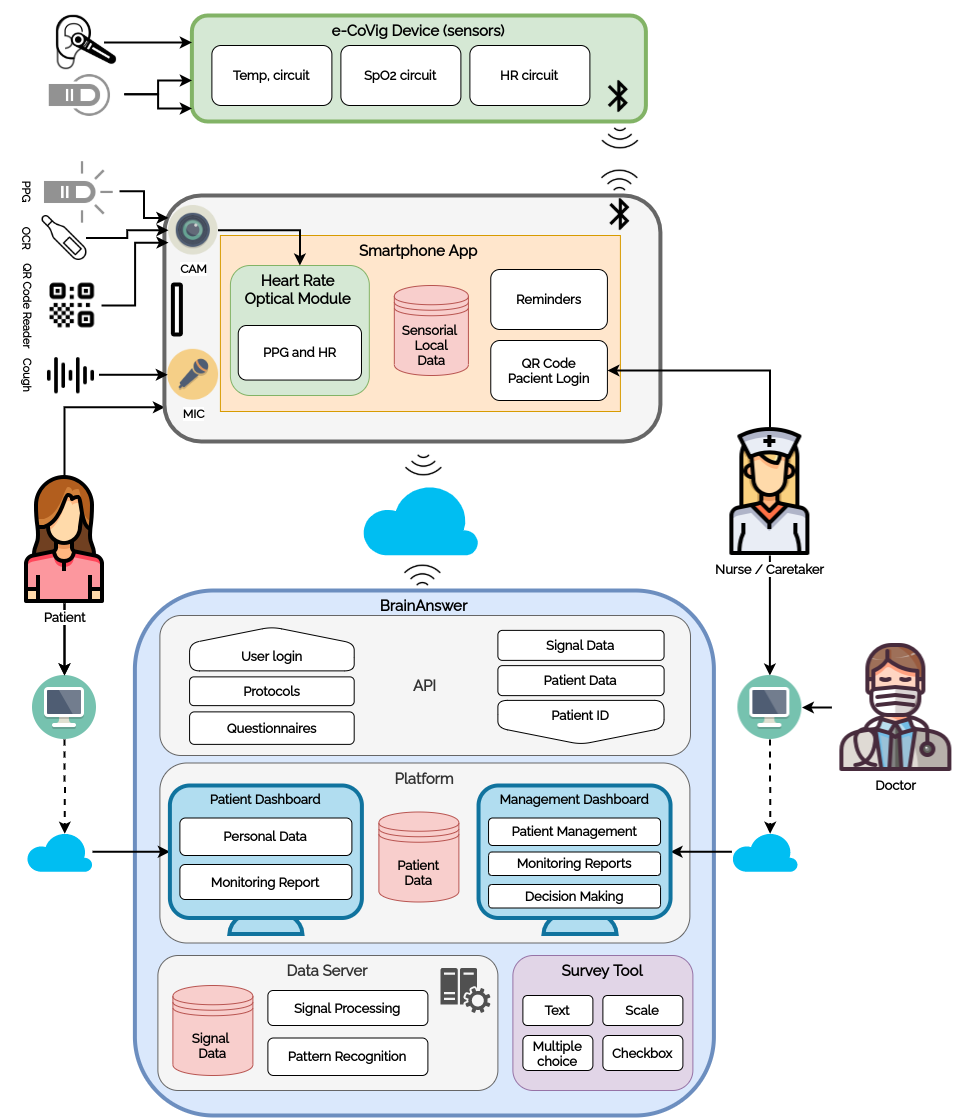
\includegraphics[width=0.75\linewidth]{images/ecovig.png}
    \caption[Diagram of e-Covig's system architecture.]{Overview of e-Covig's system architecture. Source: \cite{BrainAnswer}.}
    \label{fig:ecovig-architecture}
\end{figure}